%% This is an example first chapter.  You should put chapter/appendix that you
%% write into a separate file, and add a line \include{yourfilename} to
%% main.tex, where `yourfilename.tex' is the name of the chapter/appendix file.
%% You can process specific files by typing their names in at the
%% \files=
%% prompt when you run the file main.tex through LaTeX.
\section{Graphs and disks}
\label{sec:graphs}


\subsection{Graphs}

A graph $G$ is defined as $G = (V,E)$, where $V$ is the set of vertices and $E$ the set of edges. A vertex $v \in V$ is the fundamental unit of a graph. An edge $e \in E$ links two vertices. The vertices $vw \in V$ that $e \in E$ links are called the \textit{endpoints}.

\begin{defn}
  An embedding of a graph $G$ is a representation of this graph on the plane.
\end{defn}

A graph $G$ is planar if there is an embedding of this graph that doesn't have any crossing between the edges.

\begin{theorem}[Kuratowski]
  A graph $G$ is planar iff it doesn't contain $K_5$ or $K_{3,3}$ as a minor.
\end{theorem}


\subsection{Intersection graphs}


Given a geometric construction with multiple objects, an intersection graph is a
graph that maps the objects into vertices and every intersection between objects
is an edge between the corresponding vertices.

\begin{defn}
  A binary relation $R$ on a set $S$ is a
\end{defn}

\begin{defn}
  A poset is a partially ordered set. A partially ordered set is a binary relation
  $\leq$ over a set $A$ satisfying this axioms:
  \begin{itemize}
    \item $a \leq a$ (reflexivity).
    \item if $a \leq b$ and $b \leq a$ then $a = b$ (antisymmetry).
    \item if $a \leq b$ and $b \leq c$ then $a \leq c$ (transitivity).
  \end{itemize}
\end{defn}

\begin{defn}
  A graph $G$ is a comparibility graph if for each edge $\{u,v\} \in E$ there is
  a binary relation $R$ such that $u \leq v$ or $v \leq u$. Equivalently, $G$
  is a comparability graph if it is the comparability graph of a poset. For
  example, the Hasse diagram (figure \ref{fig:hasse}) is a comparability graph
  where the relation is inclusion.
\end{defn}

\begin{figure}
\centering

\begin{scaletikzpicturetowidth}{\textwidth}
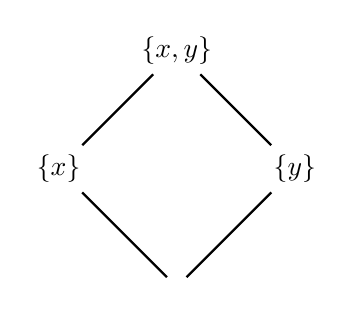
\begin{tikzpicture}[scale=1.5]
  \draw (-1cm,0cm) node (v2) {$\{x\}$};
  \draw (1cm,0cm)  node (v3) { $\{y\}$ };
  \draw (0cm,-1cm) node (v4) {$\varnothing$};
  \draw (0cm,1cm)  node (v1) {$\{x,y\}$};


  \draw[thick]  (v1) edge (v2);
  \draw[thick]  (v3) edge (v1);
  \draw[thick]  (v3) edge (v4);
  \draw[thick]  (v2) edge (v4);

\end{tikzpicture}
\end{scaletikzpicturetowidth}

\caption{Hasse diagram of a poset of the power set of 2 elements ordered by inclusion.
This graph is also a comparability graph, elements at each level are not comparable.}
\label{fig:hasse}
\end{figure}

\subsubsection{Interval graphs}

Definition of interval Graphs

Properties

Definition of MIXED interval graphs


\subsection{Realizations}

\begin{defn}
  A realization of a graph $G$ is a mapping of this graph in $\mathbb{R}^2$
  respecting some properties, i.e. 2 points are linked if and only if
  their distance equals 1 (Unit Distance Graphs).
\end{defn}

The \textit{graph realizability problem} is the problem that finds a realization
of a given length $l(e)$ for a graph $G$ (this means that the edge $e$ has to
be represented by a straight line of length $l(e)$ in $\mathbb{R}^2$).

A unit distance graph $G$ is a graph that has a realization where 2 points $u,v$
have $\text{dist}(u,v) = 1$ if and only if their respective vertices are linked.
This problem  will be shown at chapter \ref{sec:complex} to be $\exists
\mathbb{R}$-complete. If  this realization doesn't have any crossing then $G$ is a
\textit{matchstick graph}.\\

A unit disk graph $G$ is a graph that has a realization where 2 points have
$\text{dist}(u,v) \leq 1$ if and only if their respective vertices are linked.
Each point can be represented as the center of a disk of unit diameter and the
edges can be represented as the intersection of 2 disks. This class of graphs
is important for this thesis, as the Thin Strip Graphs are a sub-class of
Unit Disk Graphs (section \ref{sec:thin}). Unit Disk Graph realizability is
$\exists \mathbb{R}$-complete. We will refer to the Unit Disk Graph class as
UDG and an example of a realization can be found in the figure \ref{fig:udg}.

% Figure about the K_1,3 construction
\begin{figure}
\centering

\begin{scaletikzpicturetowidth}{\textwidth}
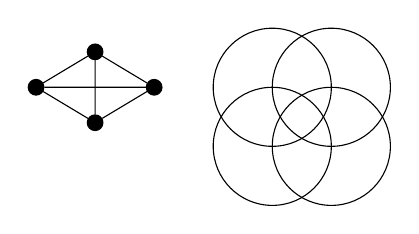
\begin{tikzpicture}[scale=1.5]

  \draw (-0.5,2.5) circle [radius=0.5];
  \draw (0,2.5) circle [radius=0.5];
  \draw (-0.5,2) circle [radius=0.5];
  \draw (0,2) circle [radius=0.5];


  \node[draw,circle,inner sep=2pt,fill,label distance=1cm] (v1) at (-2.5,2.5) {};

  \node[draw,circle,inner sep=2pt,fill,label distance=1cm] (v2) at (-2,2.2) {};
  \node[draw,circle,inner sep=2pt,fill,label distance=1cm] (v3) at (-2,2.8) {};
  \node[draw,circle,inner sep=2pt,fill,label distance=1cm] (v4) at (-1.5,2.5) {};

  \draw  (v3) edge (v2);
  \draw  (v4) edge (v1);
  \draw  (v3) edge (v1);
  \draw  (v4) edge (v2);
  \draw  (v3) edge (v4);
  \draw  (v1) edge (v2);

\end{tikzpicture}
\end{scaletikzpicturetowidth}

\caption{Realization of a UDG (Unit Disk Graph).}
\label{fig:udg}
\end{figure}
